\subsection{Materials Selection}
\subsubsection{Principles of Materials Selection}
Materials selection is the process of establishing a link between the properties required of a component and the materials available. Ashby defined materials selection in two points \cite{Ashby05}:

\begin{enumerate}
\item \textit{``Identifying the desired attribute profile and then}
\item \textit{Comparing it with those of real engineering materials to find the best match''}
\end{enumerate}
This process involves examining the requirements of the design to determine the constraints placed on the material choice; for example, a part needed high stiffness would rule out rubber from the possible materials. This narrows the large number of materials available to a smaller group of viable materials. The materials left over are ranked against their ability to fulfil the performance criteria of the design. This is done with the help of the Ashby material property charts (Figures \ref{StrengthDensity} and \ref{YmodDensity}). Finally, further attributes of the materials are considered, such as corrosion resistance or machinability, as well as the experience of the WMG technicians. This selection strategy is shown in Figure \ref{AshbyStrat} \cite{Ashby05}.

\begin{figure}[h!]
  \centering
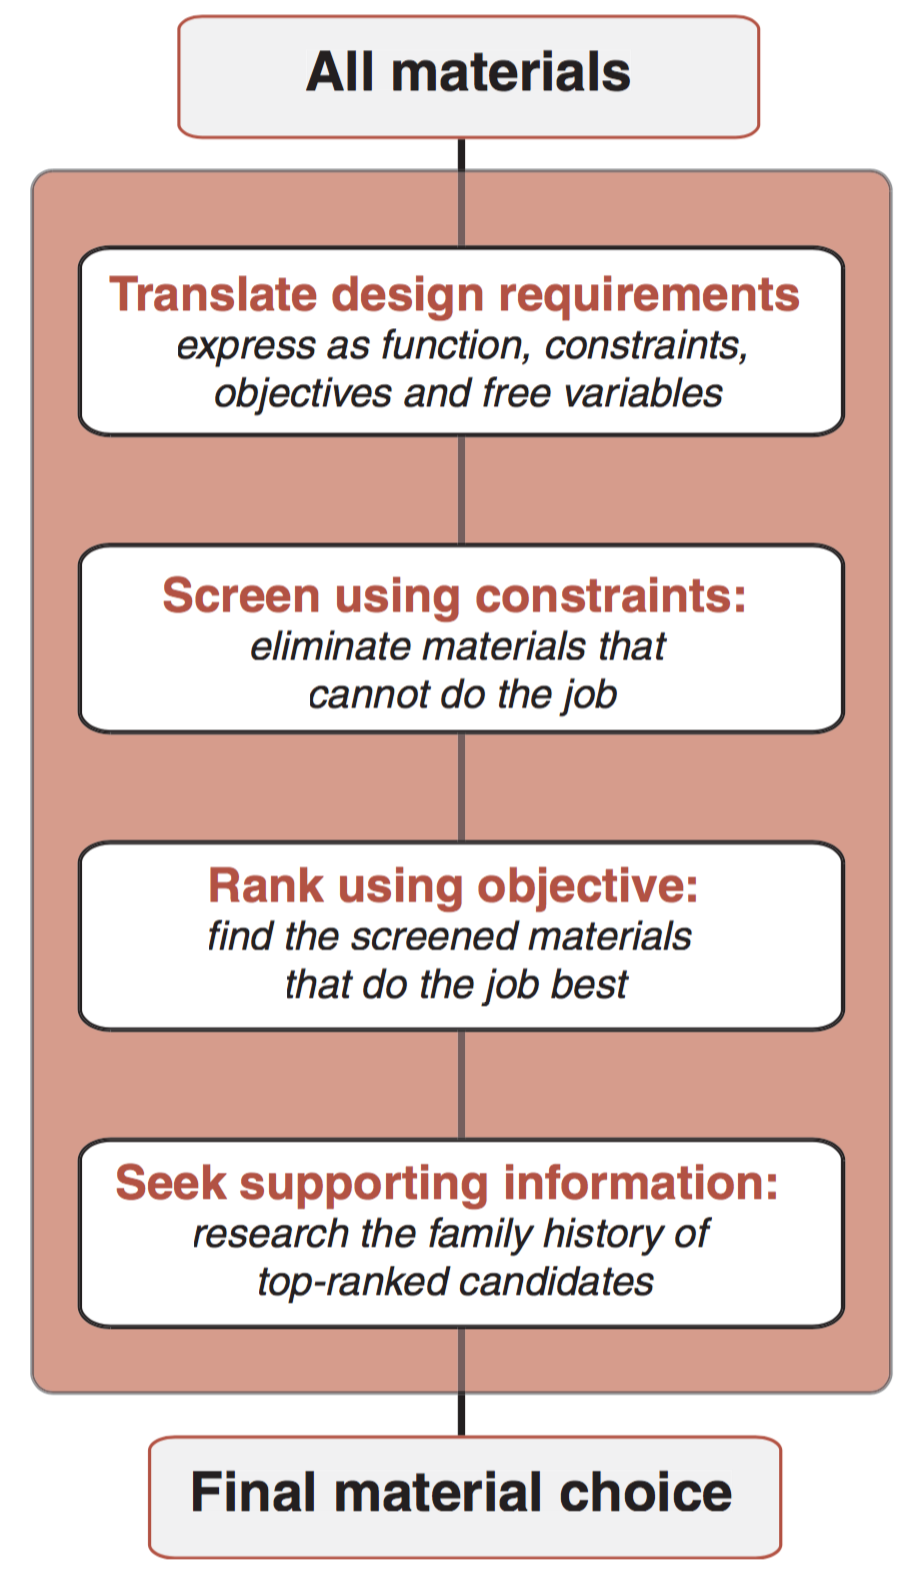
\includegraphics[width=6cm]{Images/MaxImages/AshbyStrat.png}
  \caption{Ashby Materials Selection Strategy, \cite{Ashby05}}
\label{AshbyStrat}
\end{figure}

\subsubsection{Cyclone Materials Selection using Properties Charts}
The materials selection for components of Cyclone was primarily based on the Ashby material property charts. These charts plot material properties against each other to give ratios that are invaluable for selecting a material; examples are strength-density and Young’s modulus-density. 

The desired properties for each component were considered and then the applicable Ashby chart used to determine the most appropriate materials. The most commonly used chart was that of strength against density, as high strength and low weight are required for the majority of components. The chart of Young’s modulus against density was used in tandem with strength-density as the most of the robot’s components must be stiff to withstand the stress it is subjected to during operation. 

\begin{figure}[h!]
\centering
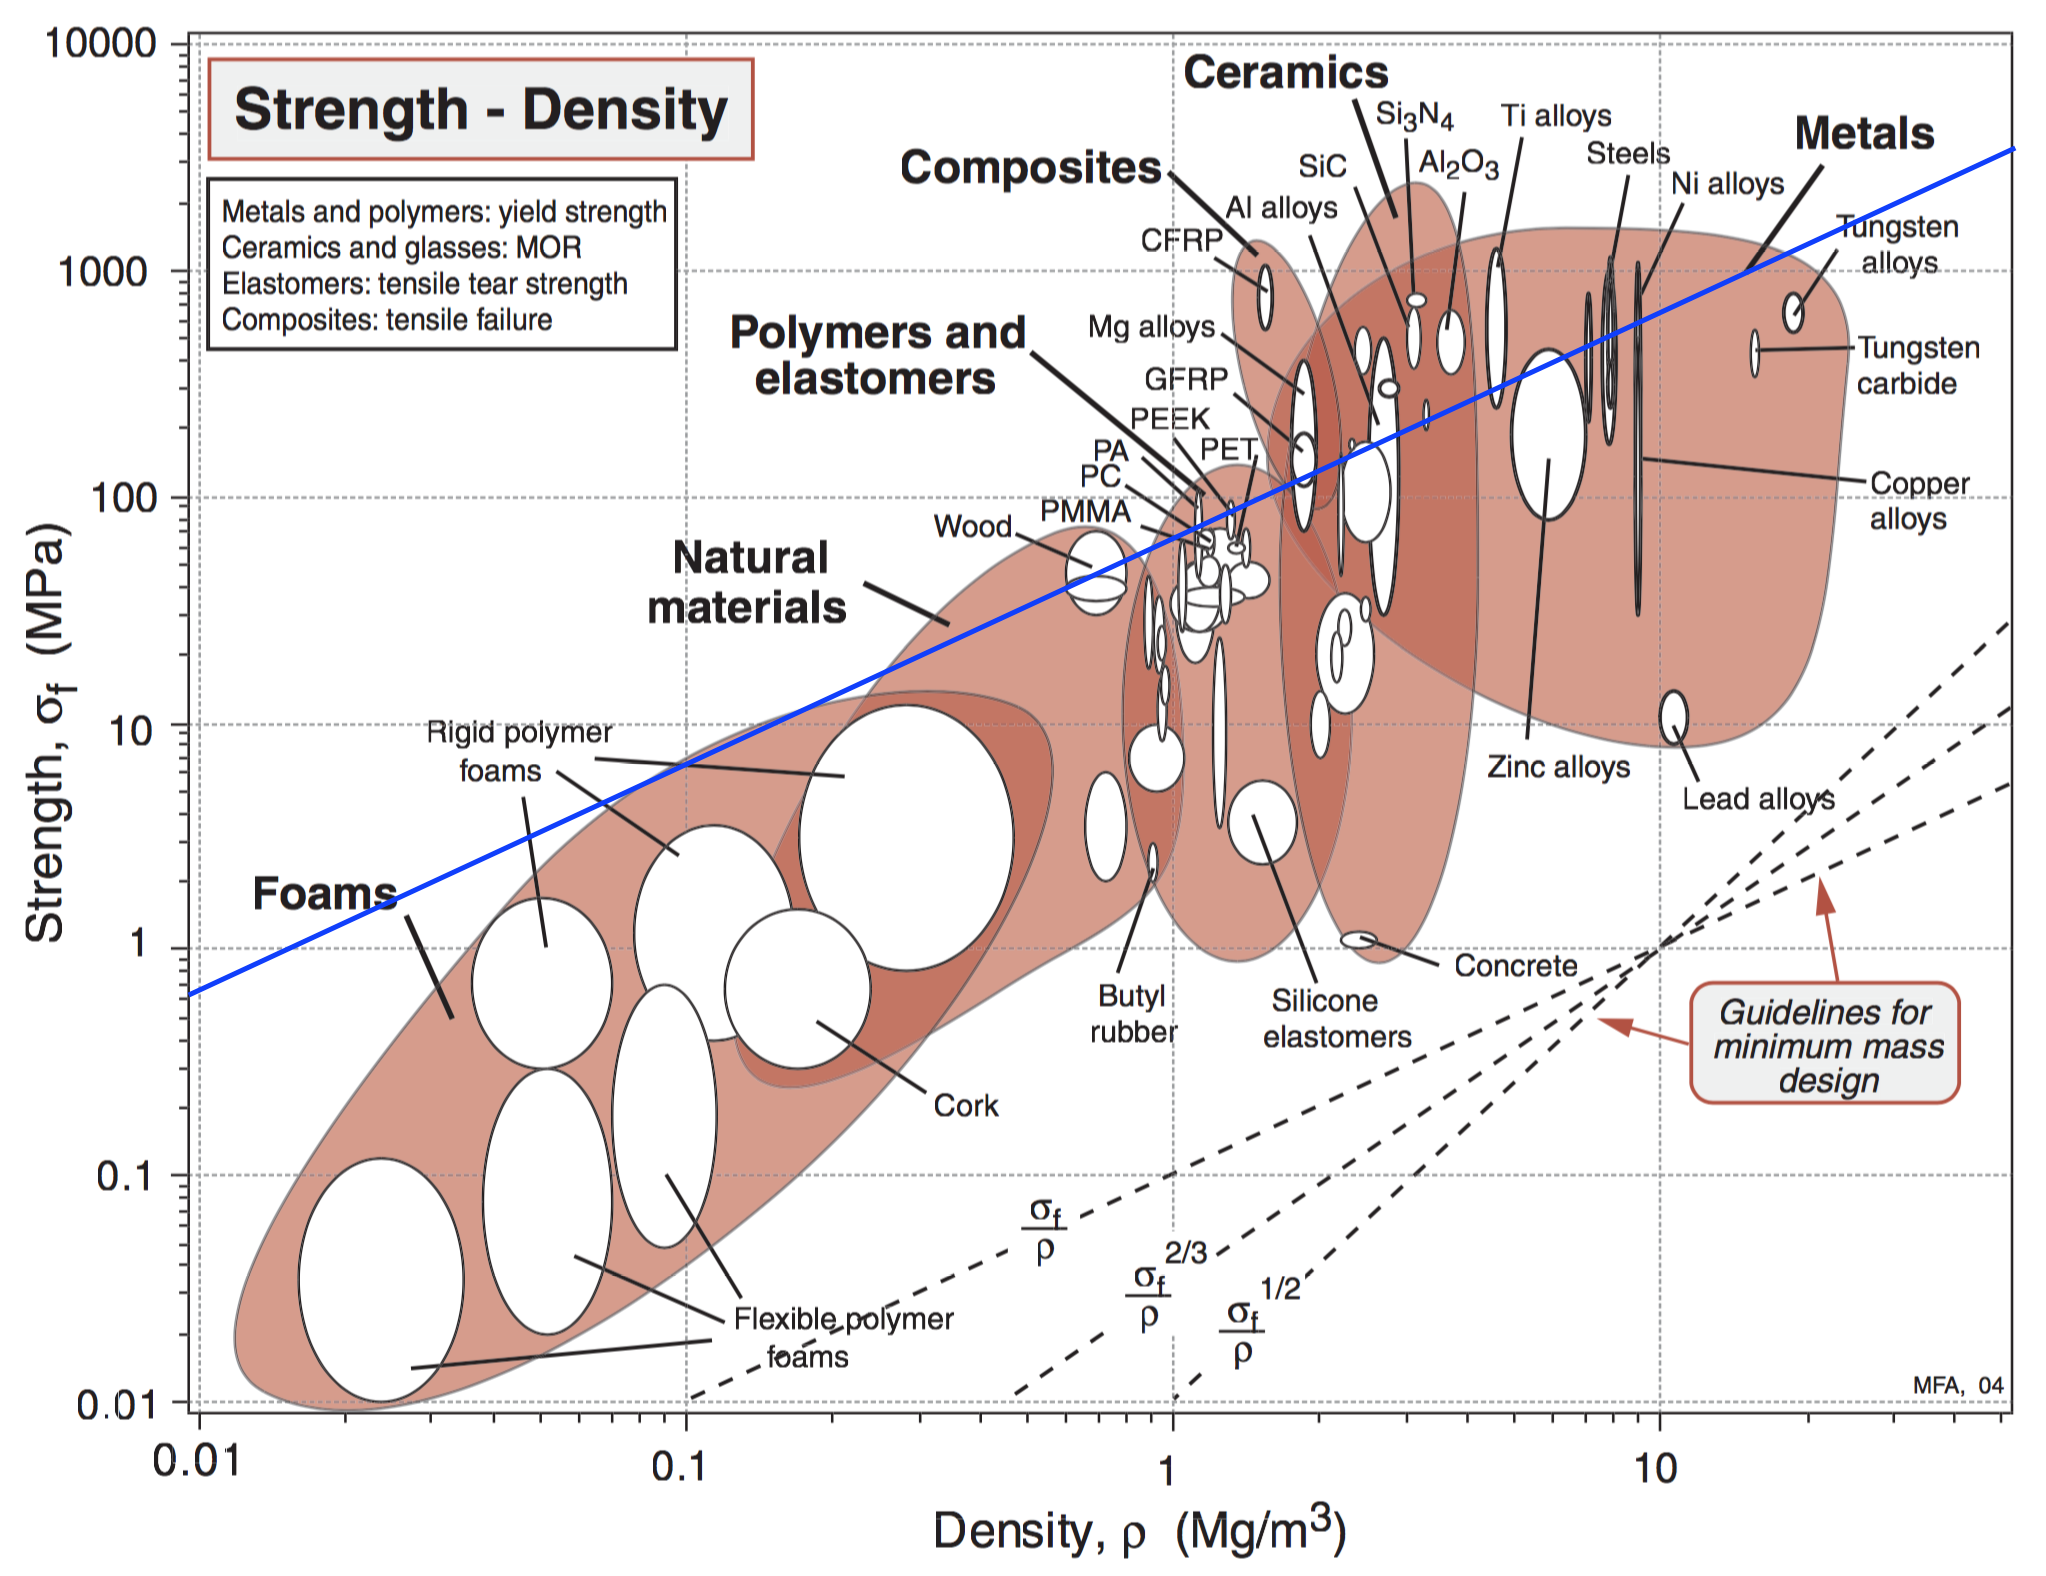
\includegraphics[width=15cm]{Images/MaxImages/StrengthDensity.png}
\caption{Ashby Strength-Density Chart, \cite{Ashby05}}
\label{StrengthDensity}
\end{figure}

\begin{figure}[h!]
\centering
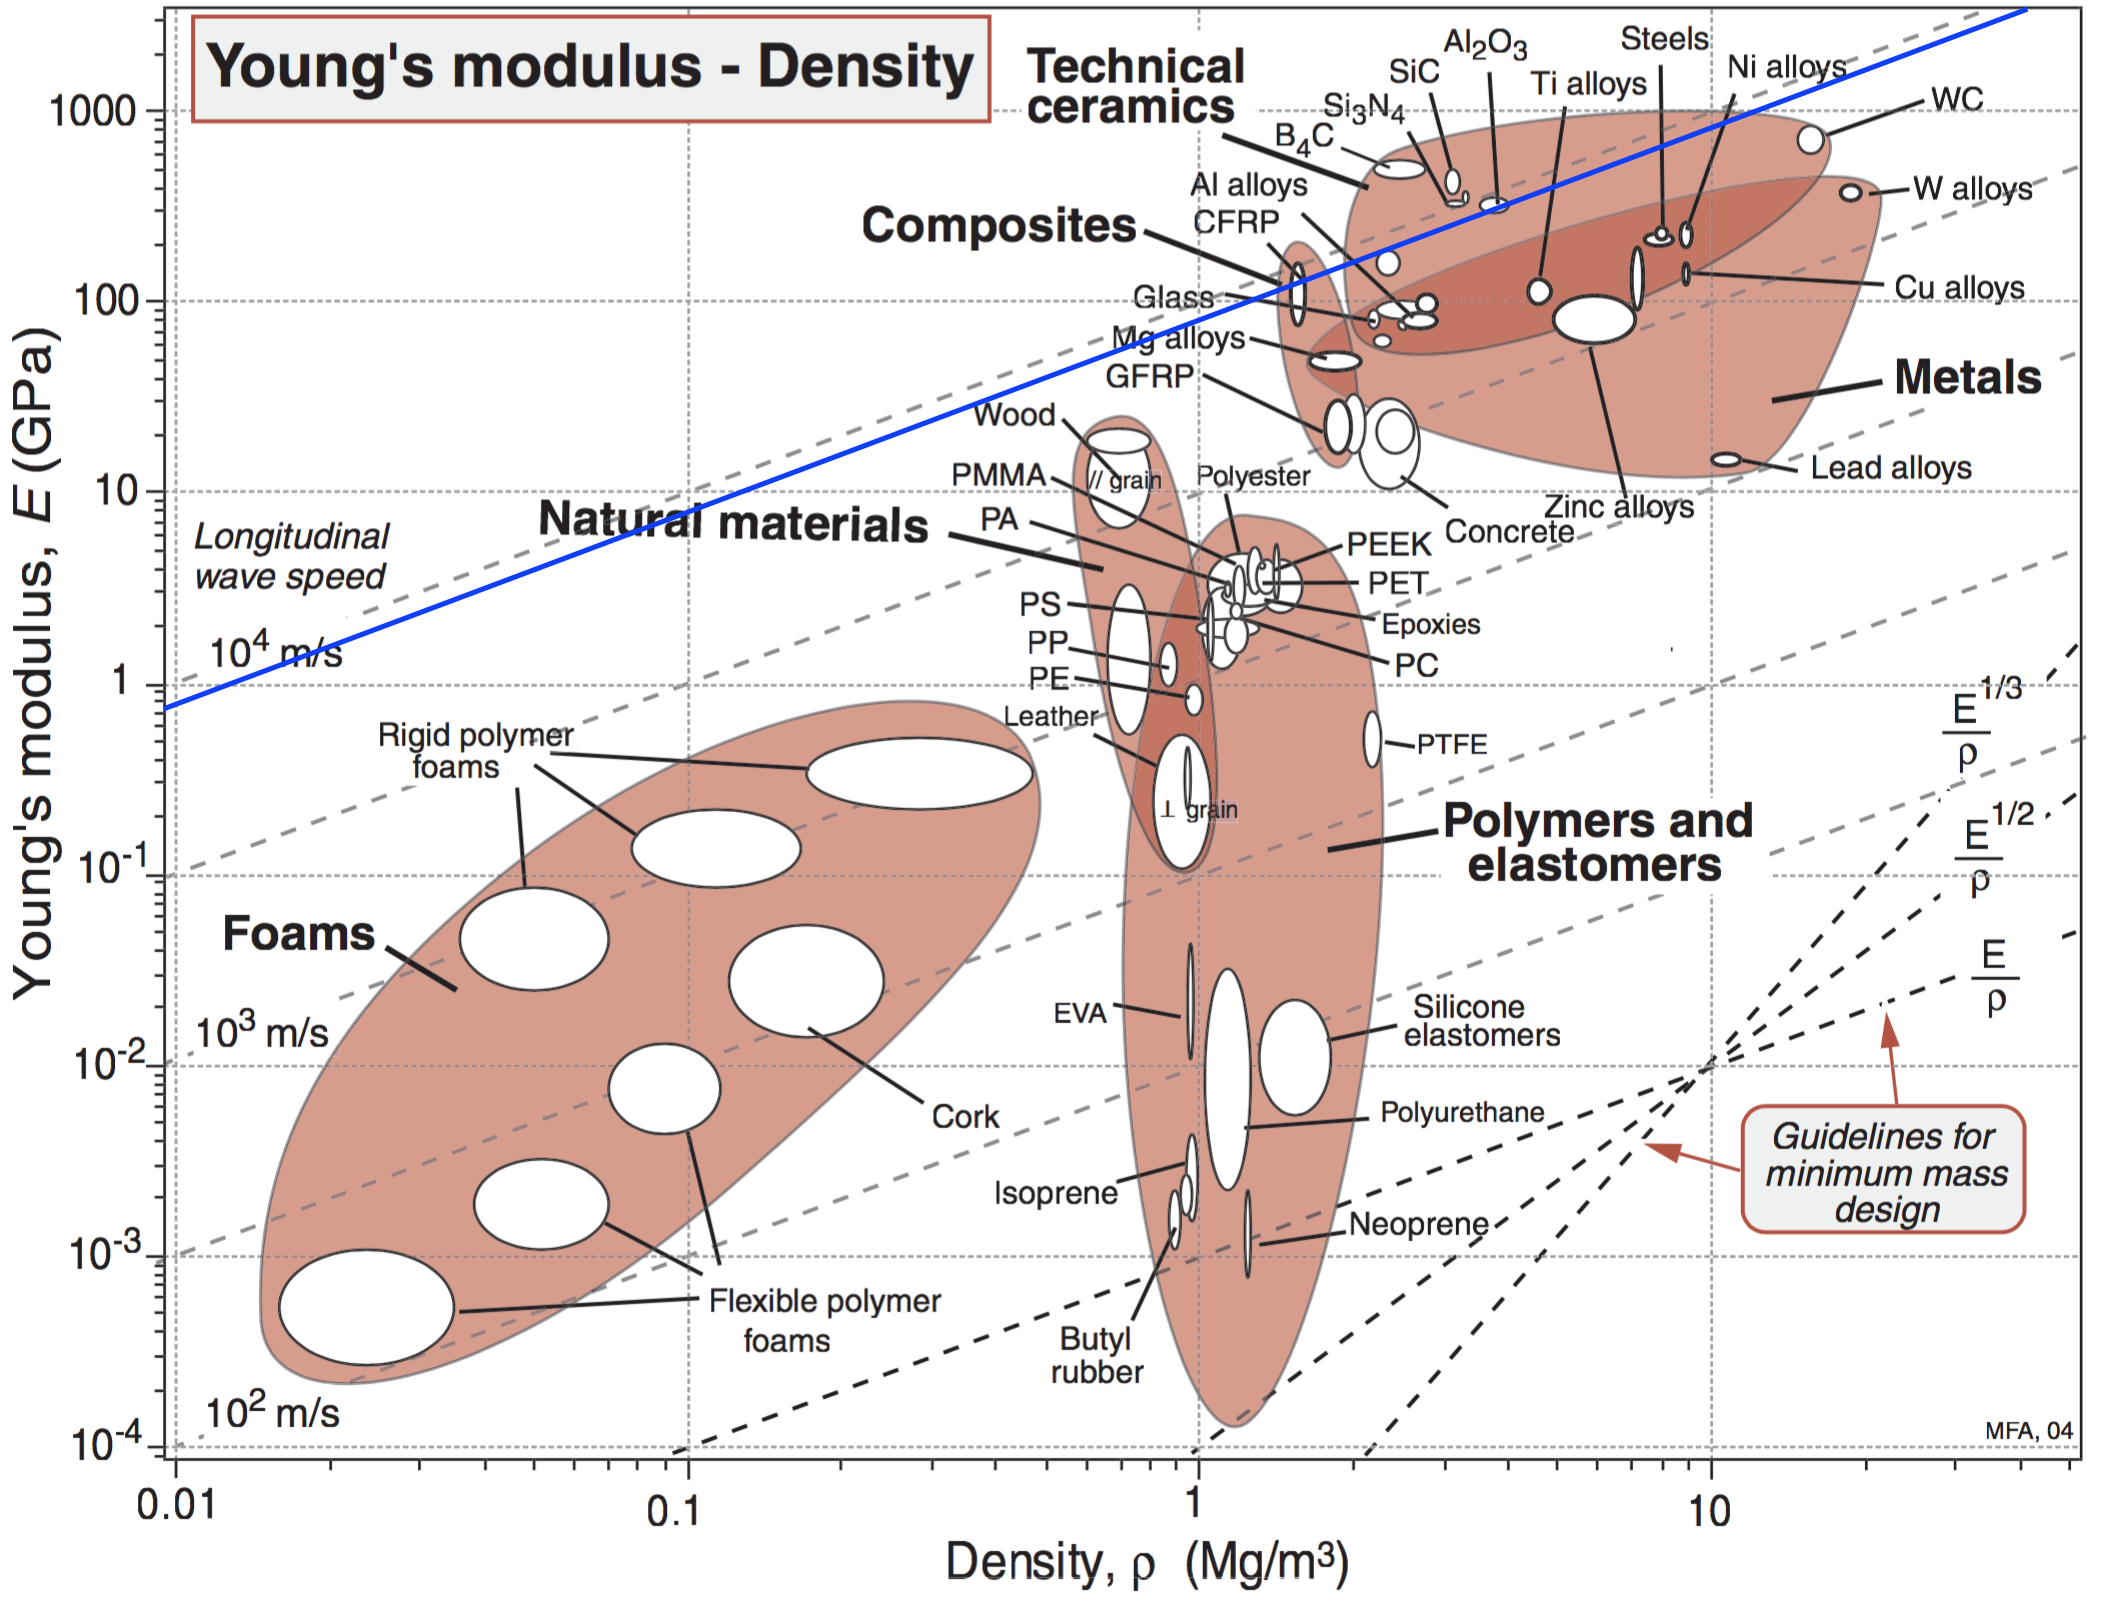
\includegraphics[width=15cm]{Images/MaxImages/YmodDensity.png}
\caption{Ashby Strength-Density Chart, \cite{Ashby05}}
\label{YmodDensity}
\end{figure}

Figures \ref{StrengthDensity} and \ref{YmodDensity} show how the Ashby charts were used to select a suitable material for the chassis. The criteria were high strength, stiffness and low weight, therefore high strength-to-weight and stiffness-to-weight was sought after. The basis material was taken to be aluminium, as it was used in for Orion’s base-plate and Makerbeam is also aluminium. The design guideline for minimum weight was moved upwards to coincide with aluminium and the other materials the line intersected evaluated for viability. Other possible materials were titanium, steels, carbon fibre reinforced plastic, nickel alloys and more. These were then ranked on further criteria. This ranking was carried out using the criteria in Table \ref{CriteriaTable}. N.B. Each attribute is ranked 1-3, the lower number represents a better material attribute. The scores for each criteria were summed and the material with the lowest overall score chosen, as it best fulfils the performance criteria of the design.

\begin{table}[]
\centering
\caption{Material Performance Criteria}
\label{CriteriaTable}
\begin{tabular}{|l|l|l|l|l|l|l|}
\hline
\textbf{Material} & \textbf{Cost} & \textbf{Availability} & \textbf{Manufacture} & \textbf{Corrosion Resistance} & \textbf{Suitability} & \textbf{Total} \\ \hline
\textbf{Al Alloy} &2&1&1&1&1&6\\ \hline
\textbf{Steel} &1&1&1&3&1&7\\ \hline
\textbf{Ni Alloy} &3&3&2&2&1&11\\ \hline
\textbf{Ti Alloy} &3&2&2&1&1&9\\ \hline
\textbf{Mg Alloy} &2&2&2&1&2&9\\ \hline
\textbf{CFRP} &3&2&3&1&3&12\\ \hline
\end{tabular}
\end{table}
\par
Material selection for some parts was carried out using different methods. For example, material selection for the torsion blades was done using the formula to calculate the length of a torsion bar for a given material's Young’s modulus. The material which had needed a length that would give a good range of adjustability was chosen, which was steel. Stainless steel was ultimately chosen for the material’s corrosion resistance, which is needed as the torsion blades are exposed to the environment on the underside of the robot.

This process was carried to determine the most appropriate material for each component. This method of materials selection is beneficial because it incorporates a scientific approach to materials selection, which is often carried out using a “gut feel” approach. Using the Ashby charts means that the most important performance criteria are considered first and all materials compared against where to give a broad range of possible materials which can then be narrowed down.